\documentclass[10pt,french]{book}
\input philippe2013

\newcounter{exoc}
\newenvironment{exoc}[1]{%
  \refstepcounter{exoc}\textbf{Exercice \theexoc} :\hfill {\textbf{#1}}\par
  \medskip}%
{\medskip}

\begin{document}

\pagestyle{empty}

\begin{center}
\renewcommand\arraystretch{1.5}
\begin{tabularx}{\textwidth}{|>\centering m{2.5cm}|>\centering X|>{\centering\arraybackslash} m{2.5cm}|}
	\hline
		1\iere \bsc{e.e.a.c.} & Lundi 3 février \np{2014} & \textbf{Complexes Probabilités} \\
	\hline
		\multicolumn{3}{|c|}{\bsc{Contrôle de mathématiques}} \\
	\hline
        \multicolumn{1}{|r}{\bsc{Nom}:} & \multicolumn{2}{l|}{} \\
		\multicolumn{1}{|r}{Prénom:} & \multicolumn{2}{l|}{} \\
	\hline
        \multicolumn{3}{|l|}{\bfseries Note et observations :} \\[1cm]
    \hline
\end{tabularx}\bigskip
\renewcommand\arraystretch{1}

{\itshape
La qualité et la précision de la rédaction seront prises en compte dans l'appréciation des copies.\par
Le barème est indicatif.}
\end{center}

\begin{exoc}{1 + 1 = 2 points}
\begin{enumerate}
    \item \'Ecrire le nombre $z$ suivant sous forme algébrique :
        \[z = \intervalleff{12}{\dfrac{\pi}{6}}\]
    \item \'Ecrire le nombre $z'$ suivant sous forme trigonométrique :
       \[z' = 2 - 2\I \sqrt 3\]
\end{enumerate}
\end{exoc}\[*\]

\begin{exoc}{1 + 2 + 3 + 1 + 1 = 8 points}
    On considère les nombres complexes suivants :
        \[z_A = \sqrt 3 + \I \qq z_B = z_A - 4\I \qetq z_C = 3 \overline{z_A} + 2\I.\]
    \begin{enumerate}
        \item \'Ecrire sous forme algébrique les nombres $z_B$ et $z_C$.
        \item On désigne par $A$, $B$ et $C$ les points images respectifs des nombres $z_A$, $z_B$ et $z_C$ dans un repère orthonormé direct \Ouv.
        \begin{enumerate}
            \item En détaillant précisément la démarche, démontrer que le triangle $ABC$ est équilatéral.
            \item \'Ecrire $z_A$ et $z_B$ sous forme trigonométrique.
            \item En utilisant une formule du cours et en détaillant précisément les étapes, déterminer la mesure de l'angle $\left(\vect{OB} \pv \vect{OA}\right)$.
            \item En déduire alors la nature exacte du triangle $OAB$. Justifier la réponse.
        \end{enumerate}
    \end{enumerate}
\end{exoc}

\vfill

\begin{center}
    \bfseries Tourner la page !
\end{center}\clearpage

\begin{exoc}{1,5 + 3,5 = 5 points}
    Soient $A$ et $B$ deux événements. On rappelle la formule suivante :
    \[p(A) + p(B) = p(A \cup B) + p(A \cap B).\]
    Dans un groupe de $250$ personnes, $100$ sont des femmes, $30$ sont des femmes exerçant la profession de chef d'entreprise et $120$ des personnes du groupe sont des chefs d'entreprise.\par
    On choisit au hasard une personne du groupe.\par
    On note $F$ et $C$ les événements suivants :\par
    $F$ : << la personne est une femme >>.\par
    $C$ : << la personne est chef d'entreprise >>.
    \begin{enumerate}
        \item En détaillant les calculs, déterminer $p(F)$, $p(C)$ et $p\left(\overline F\right)$. Donner les résultats \textbf{sous forme décimale}.
        \item Pour chacun des événements suivants, donner une description par une phrase simple puis déterminer \textbf{sous forme décimale} leur probabilité en justifiant précisément :
            \[C \cap F \qq C \cup F \qq \overline C \cap F \]
    \end{enumerate}
\end{exoc}\[*\]

\begin{exoc}{1,5 + 1 + 1,5 + 1 = 5 points}
\begin{minipage}{0.7\linewidth}
    Grâce à un système de détecteur, une borne de péage automatique peut délivrer des tickets à deux hauteurs différentes, selon le véhicule détecté, afin que le conducteur ne soit pas obligé de sortir de sa voiture.\par
    S'il s'agit d'une voiture, d'une moto ou d'une camionnette, le ticket sort en bas.\par S'il s'agit d'un camion, le ticket sort en haut.\par
    La société d'autoroute a étudié que l'une de ces bornes étaient défectueuses : de temps en temps, le ticket ne sort pas à la bonne hauteur, de façon indépendante pour chaque véhicule. D'après l'étude, la probabilité que le conducteur ne soit pas obligé de sortir de la voiture est égale à $0,9$.
\end{minipage}\qquad
\begin{minipage}{0.25\linewidth}
    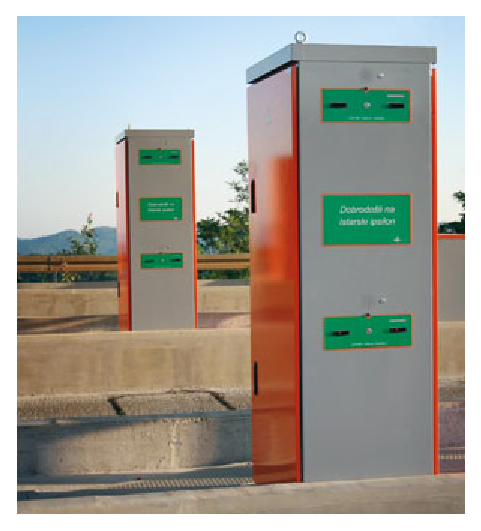
\includegraphics[width=0.95\linewidth]{peage.eps}
\end{minipage}

    \begin{enumerate}
        \item On observe le comportement de la borne lors du passage de trois véhicules.\par Expliquer \textbf{précisément} pourquoi on peut modéliser la situation avec un schéma de Bernoulli.
        \item On appelle $A$ l'événement : << aucun conducteur n'est obligé de descendre de son véhicule pour récupérer le ticket >>. Calculer $p(A)$.
        \item On appelle $B$ l'événement : << un seul conducteur exactement descend de son véhicule pour récupérer le ticket >>. Calculer $p(B)$.
        \item On appelle $C$ l'événement : << au moins un conducteur descend de son véhicule pour récupérer le ticket >>.\par
        La société d'autoroute doit changer la borne défectueuse lorsque $p(C) \geqslant 25\%$.\par
        La borne étudiée doit-elle être changée ? Justifier précisément la réponse.
    \end{enumerate}
\end{exoc}

\end{document} 